%\documentclass[12pt, answers]{exam}
\documentclass[12pt]{exam}
%\setlength{\textheight}{5in}
%\usepackage[textwidth=9in,centering]{geometry}
\usepackage[a4paper, margin=1in]{geometry}
\usepackage{econometrics}
\usepackage{lmodern}
\usepackage{amssymb,amsmath,amsfonts,amsthm,enumerate,enumitem}
\usepackage{setspace, graphicx, multirow, dcolumn, caption}
\usepackage{bm, booktabs}
\pagestyle{empty}

\firstpagefooter{}{Page \thepage\ of \numpages}{}
\runningfooter{}{Page \thepage\ of \numpages}{}

% \usepackage{etoolbox}
% \AtEndEnvironment{question}{\bigskip\bigskip}

% \usepackage{etoolbox}
% \makeatletter
%  \patchcmd\@setheadheight{\endgroup}{\global\vsize=\textheight\endgroup}{}{}
% \makeatother


% Notation
\def\eps{\varepsilon}
\def\var{\text{Var}}
\def\cov{\text{Cov}}
\def\corr{\text{Corr}}
\def\Ybar{\overline{Y}}
\def\Xbar{\overline{X}}
\def\ybar{\overline{y}}
\def\xbar{\overline{x}}
\def\Yhat{\widehat{Y}}
\def\yhat{\widehat{y}}
\def\fhat{\widehat{f}}
\def\bhat{\widehat{\beta}}
\def\betahat{\widehat{\vbeta}}
\def\MSE{\text{MSE}}
\def\SE{\text{SE}}
\def\train{\mathcal{T}}
\def\data{\mathcal{D}}
\def\model{\mathcal{M}}
\def\hvtheta{\widehat{\vtheta}}
\def\({\left(}
\def\){\right)}



\makeatletter
\g@addto@macro\@floatboxreset\centering
\makeatother



\setlength{\parindent}{0pt}
\onehalfspace

%\renewcommand{\labelitemi}{1.}

%\bracketedpoints
\pointpoints{mark}{marks}
% \qformat{\textbf{Problem \thequestion: \\ \hspace{10pt} \\}}


\qformat{
    \textbf{Question \thequestion \hspace{2pt} \thepoints}
    \hfill
    \vrule depth 20pt width 0pt % Large depth to make space
}

\bonusqformat
{
    \textbf{Question \thequestion \hspace{2pt} \thepoints}
    \hfill
    \vrule depth 20pt width 0pt % Large depth to make space
}

\bonuspointpoints{mark, bonus)}{marks, bonus}


\begin{document}



\begin{center}
{\Large \textbf{QBUS6810} \\\textbf{Statistical Learning and Data Mining}}\\  \large{Tutorial 13 (Written Exercises)}
\end{center}




\begin{questions}

\question

Suppose that you want to train a Naive Bayes classifier for the following data.

\medskip

\begin{center}
\begin{tabular}{ll|l}
\toprule
\multicolumn{2}{c}{\textbf{Inputs}}      &          \multicolumn{1}{c}{\textbf{Output}}   \\
\multicolumn{1}{c}{Salary ($X_1$)} & \multicolumn{1}{c}{Salary of the spouse ($X_2$)} & \multicolumn{1}{c}{Happy (H)}\\ \midrule
80          & 60         & Yes ($1$)    \\
100          & 80         & Yes ($1$)    \\
70          & 80   & No ($0$)   \\
50          & 20   & No ($0$)   \\ \bottomrule
\end{tabular}
\end{center}

\medskip

The unit of measurement for Salary is \$1K.

\bigskip

\begin{parts}

\part Assume that the distribution of Salary given the value of H is Gaussian, i.e. the class conditional densities for $X_1$ are:
\begin{align*}
p(x_1|H=h)=\frac{1}{\sqrt{2\pi\sigma^2_{1h}}}\exp\left(-\frac{\(x_1-\mu_{1h}\)^2}{2\sigma^2_{1h}}\right),\quad \text{for}\; h=0\;\text{and}\; h=1.
\end{align*}
Estimate (using the data) the means $\mu_{1h}$ and the variances $\sigma^2_{1h}$ for $h=0$ and $h=1$.  Show your work.


\part Assume that the distribution of the Salary of the spouse given the value of H is also Gaussian, i.e. the class conditional densities for $X_2$ are:
\begin{align*}
p(x_2|H=h)=\frac{1}{\sqrt{2\pi\sigma^2_{2h}}}\exp\left(-\frac{\(x_1-\mu_{2h}\)^2}{2\sigma^2_{2h}}\right),\quad \text{for}\; h=0\;\text{and}\; h=1.
\end{align*}
Estimate (using the data) the means $\mu_{2h}$ and the variances $\sigma^2_{2h}$ for $h=0$ and $h=1$.  Show your work.


\part Estimate  (using the data) the class probabilities: $P(H=1)$ and $P(H=0)$.


\part Derive the Naive Bayes classifier estimate of the probability\\ $P(H=1|X_1=x_1,X_2=x_2)$, first using the general formulas, and then incorporating your specific results from parts (a), (b), and (c).

\end{parts}

\clearpage

\question

Suppose $X_1$ and $X_2$ take values in the interval $[0,10]$.

\begin{parts}

\part

Consider the following regression tree.  The numbers next to the terminal nodes give the corresponding predicted values.

\begin{figure}[!ht]
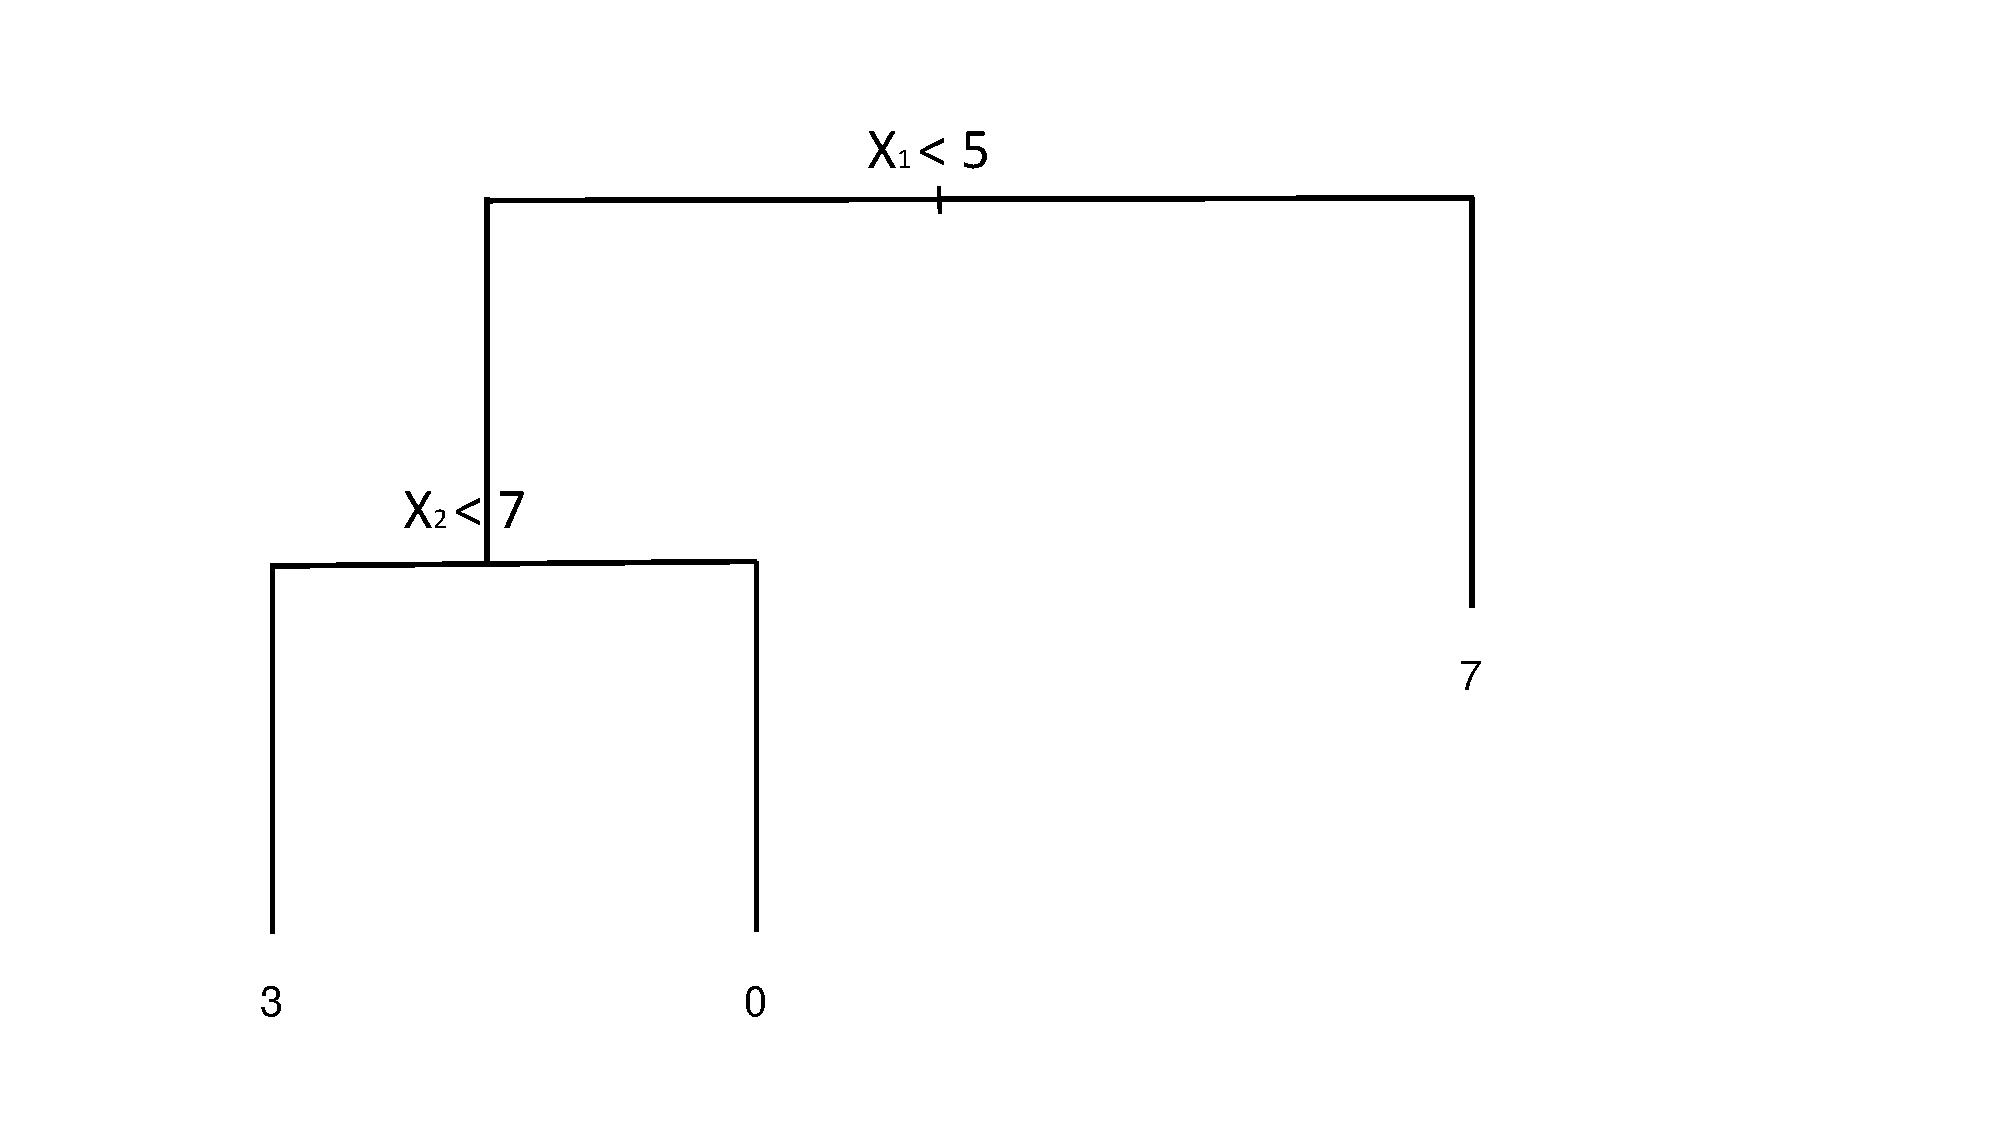
\includegraphics[scale=0.4]{T1.pdf}
\end{figure}

Sketch the corresponding partition of the predictor space.  Write the predicted values inside the corresponding regions of the partition.


\part

Now consider the following partition of the predictor space.

\begin{figure}[!ht]
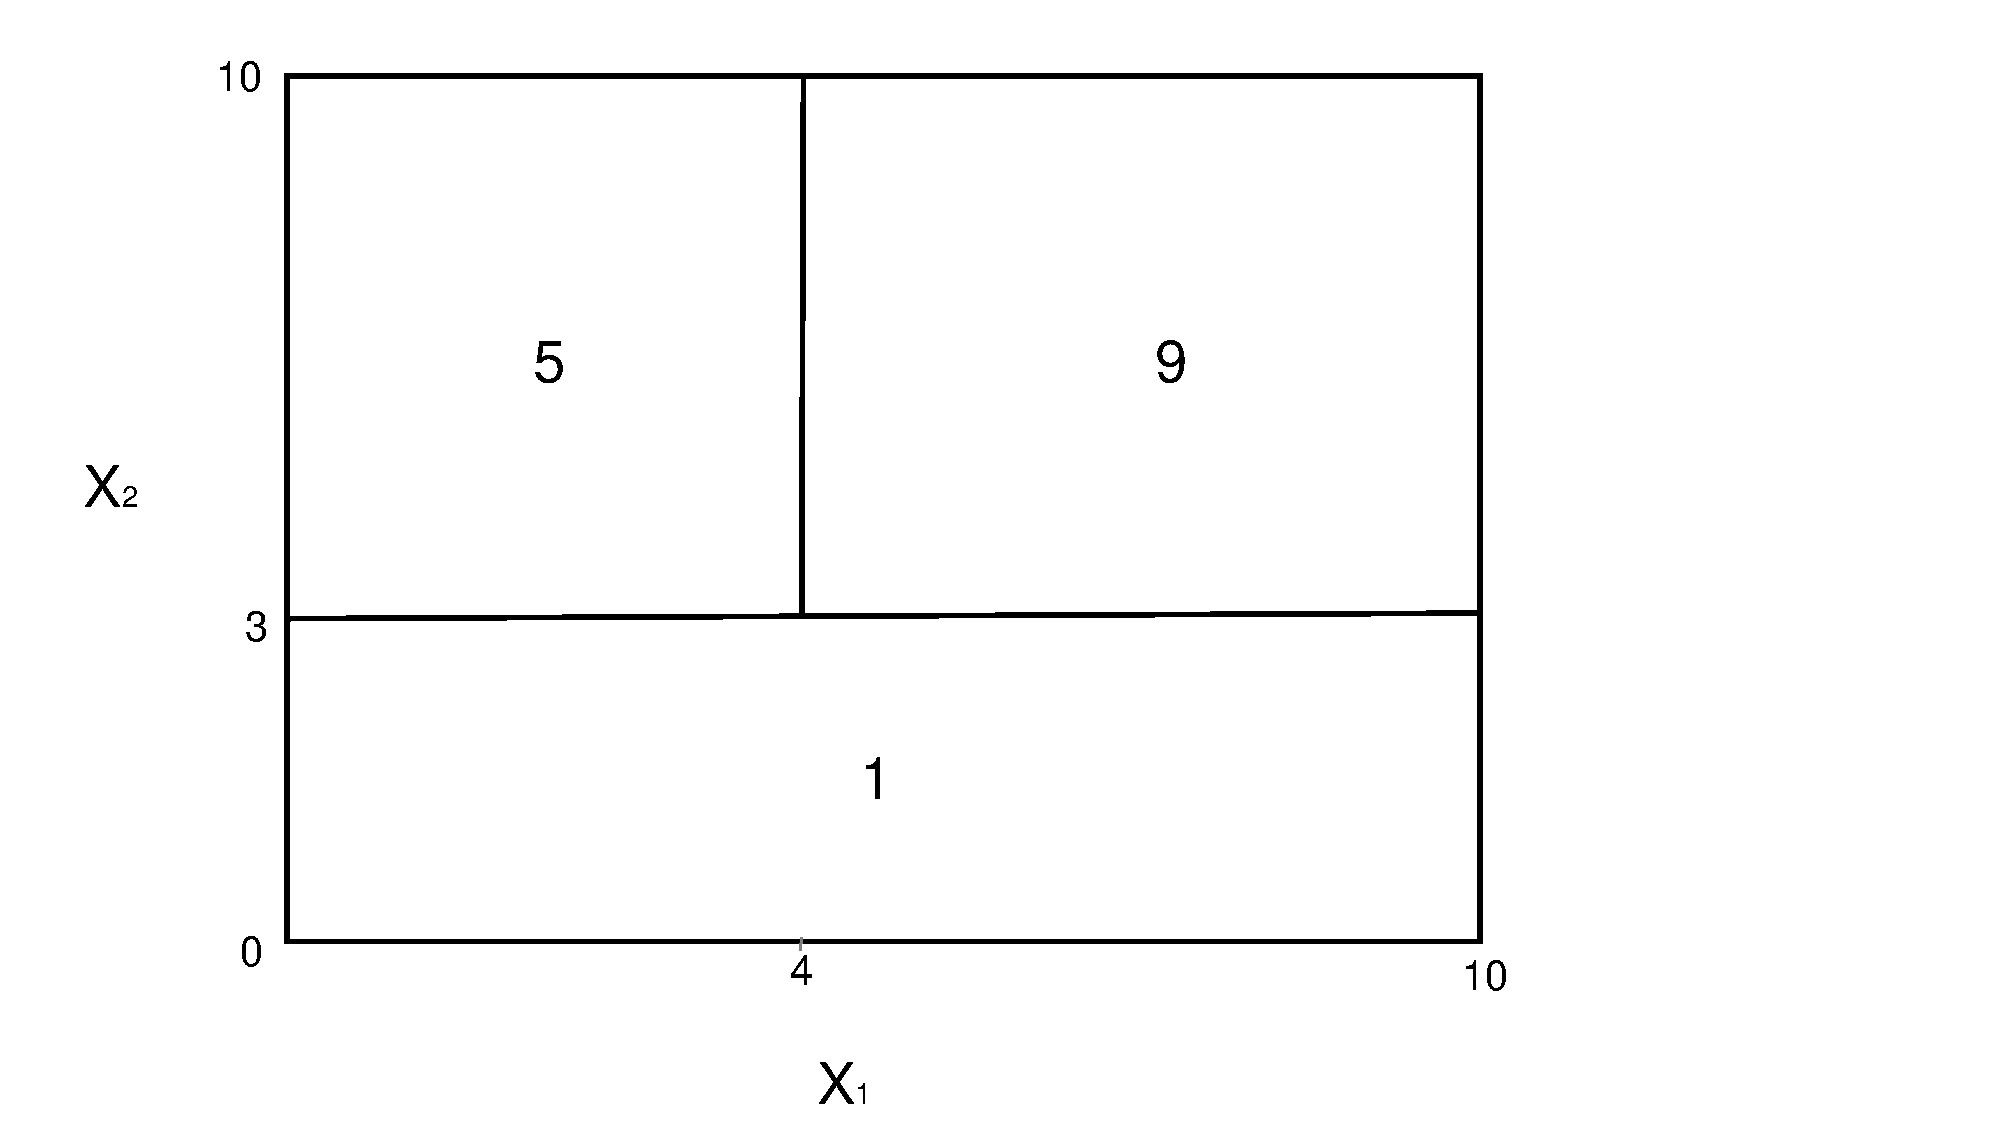
\includegraphics[scale=0.4]{P2.pdf}
\end{figure}

Create a diagram for the corresponding regression tree.

\part For the tree in part (b), write down the estimated regression function, $\widehat{f}(x_1,x_2)$.  Does this function correspond to a GAM (i.e. an additive model) or a model with interactions?


\end{parts}


\end{questions}

\end{document} 